\section{Evaluation of database}\label{subsec:evaluation-db}

According to \cite{flask_book2018}, \ac{sql} databases are a good choice for efficiently storing structured data.
This is because their paradigm \acs{acid}, i.e. \acl{acid}, provides high reliability.
\ac{nosql} databases, on the other hand, are more flexible and can be used to store unstructured data \cite{flask_book2018}.
They do not require a predefined schema and can therefore accept documents of arbitrary structure \cite{flask2018}.

Usually, \ac{nosql} databases do not offer services such as \texttt{JOIN} \cite{flask2018}.
According to \citeauthor{flask2018}, \ac{nosql} databases make a tradeoff between storage and speed, as well as a tradeoff between consistency and availability.
\ac{nosql} databases are said to outperform out-of-the-box \ac{sql} databases \cite{flask2018}.

% separation of initialisation and insertion
The time per step is shown in \autoref{fig:time_init_db}.
Separating the initialization into multiple steps is beneficial since it is possible to update the embeddings without having to recreate the database.
Moreover, the time per step facilitates debugging and comparing the models used to create the embeddings.

\begin{figure}[htp] % htp = hier (h), top (t), oder auf einer eigenen Seite (p).
    \centering
    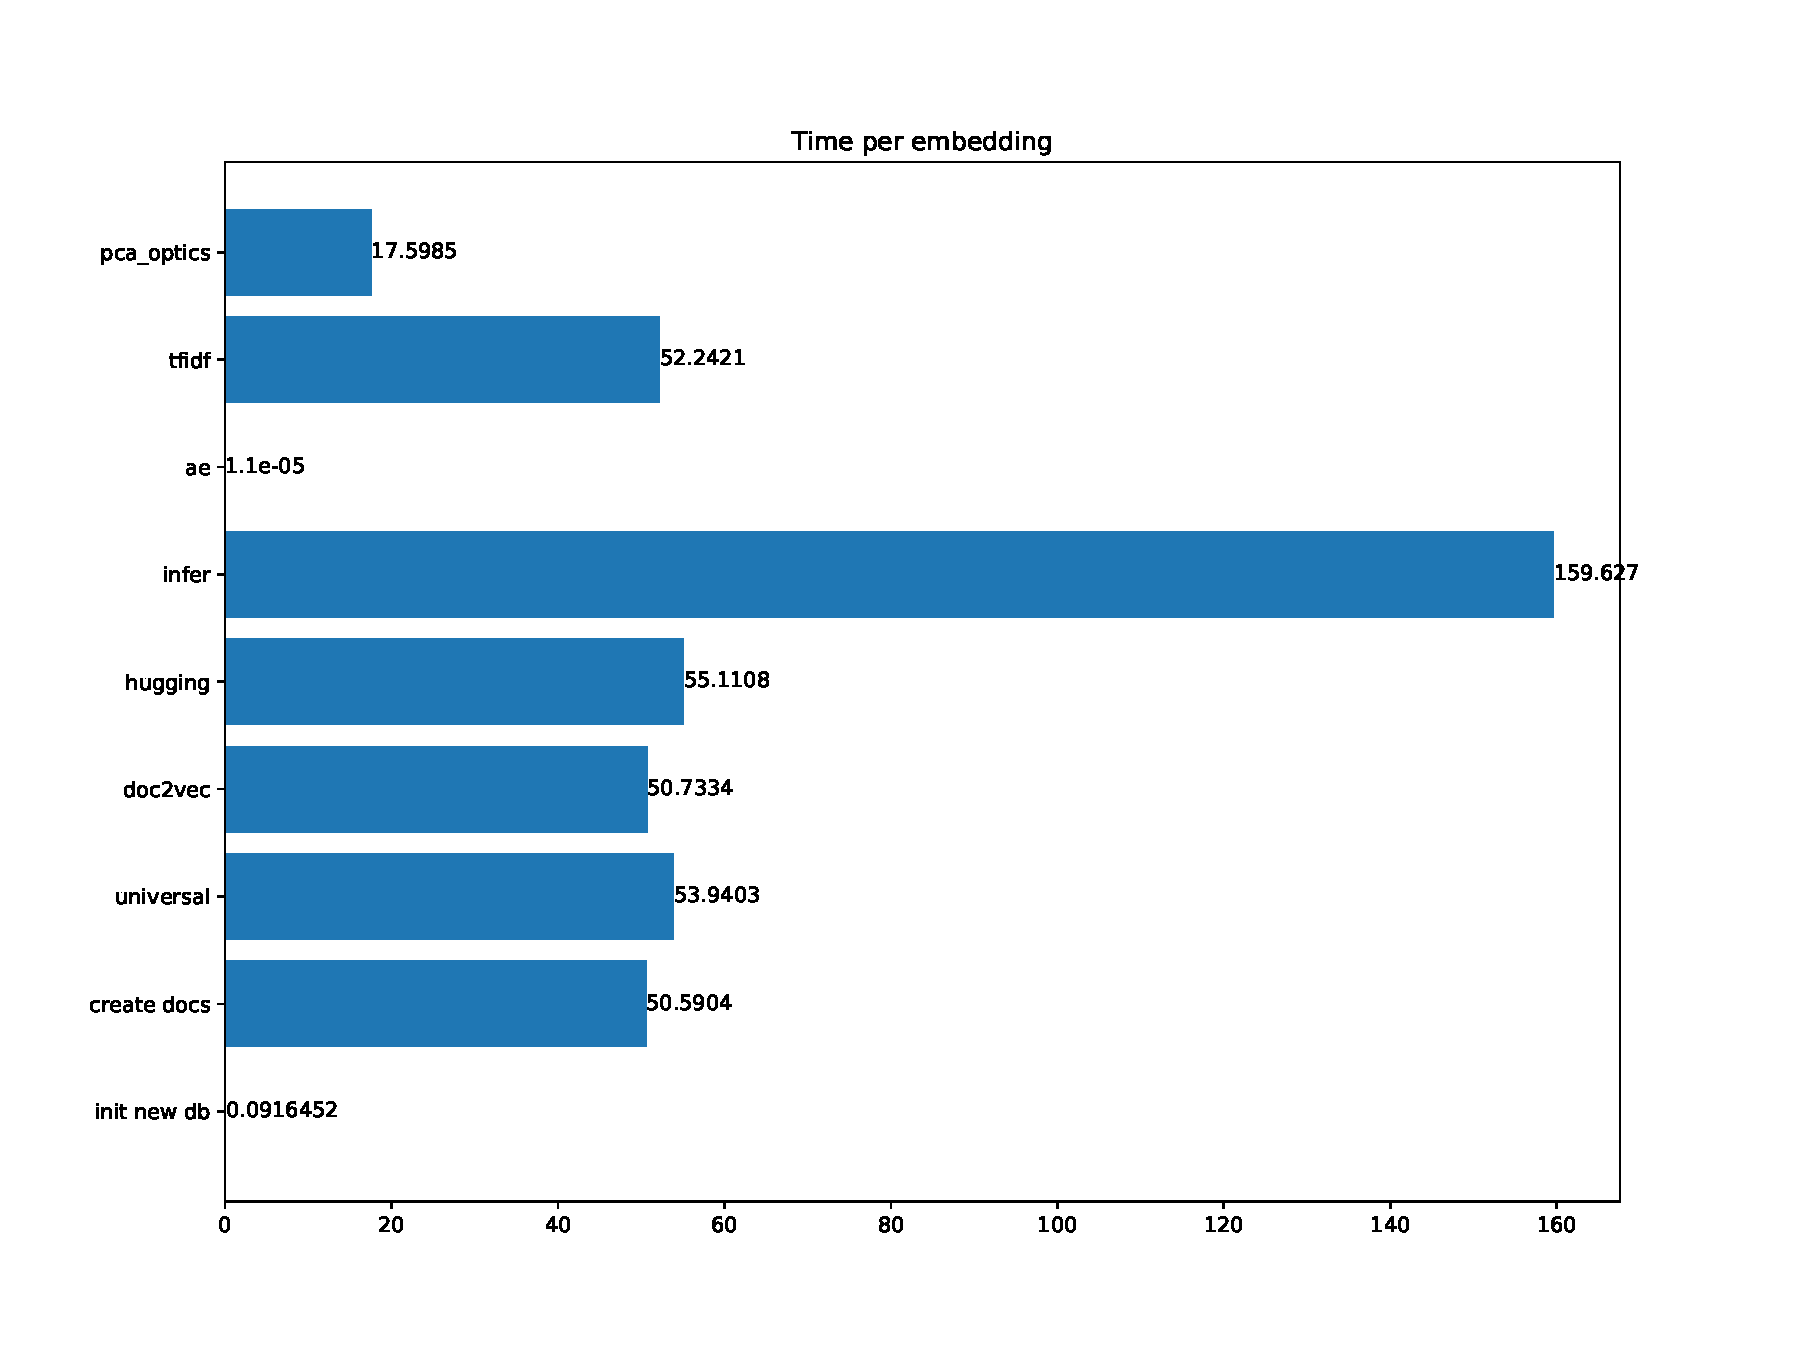
\includegraphics[width=0.6\textwidth]{images/Elasticsearch/time_per_emb.pdf}
    \caption{Time per step when creating the Bahamas database using a selection of 195 documents.
    The time was measured using the \texttt{timer} from \texttt{timeit.default\_timer} on a Apple M2 Pro MNW83D/A with 16 \ac{gb} RAM and 12 cores.
    }
    \label{fig:time_init_db}
\end{figure}

% similarity
Since the similarity between vectors is usually calculated using some form of cosine similarity, 
rather than Euclidean distance in literature, cosine is preferred over Euclidean distance. 
Since the models may produce embeddings, which are not normalized, the cosine similarity is used instead of the dot product.
Soft cosine similarity is not used, since it is not available in \databaseName{}.
\textcolor{red}{soft cosine would be better!}

A document store database can be used if the primary goal is to write fast rather than write save \cite{flask2018}.